% !TeX program = lualatex -synctex=1 -interaction=nonstopmode --shell-escape %.tex
\documentclass[international_finance_p1.tex]{subfiles}
\begin{document}
\setbeamercovered{transparent}
\section{The Balance of Payments (BoP)}
\subsection{The BoP components}
\begin{frame}{}
\begin{itemize}[<+->]
\item
Balance of payments accounts are an accounting record of all monetary transactions between a country and the rest of the world.
\item
Balance of payments data are reported quarterly for most developed countries.
\item
If any particular account has the value of the credit entries that exceeds the debits, the account has a surplus. If the debits exceed the credits, a deficit exists.
\item
A surplus or deficit can apply only to a particular account of the balance of payments.
\item
The balance of payments is always zero.
\end{itemize}
\end{frame}
\begin{frame}{Balance of payments in the IMF`s terminology}
\begin{itemize}[<+->]
\item
The current account includes the value of trade in merchandise, services, investment income, and cash transfers.
\item
The capital account represents transfers. Transfers are one-way flows, such as gifts, as opposed to commercial exchanges (i.e., buying/selling and barter).
\item
The financial account is the net change in ownership of foreign assets. It includes loans, direct and portfolio investments between the country and the rest of world, reserve account.
\end{itemize}
\end{frame}
\begin{frame}{Every country’s major export}
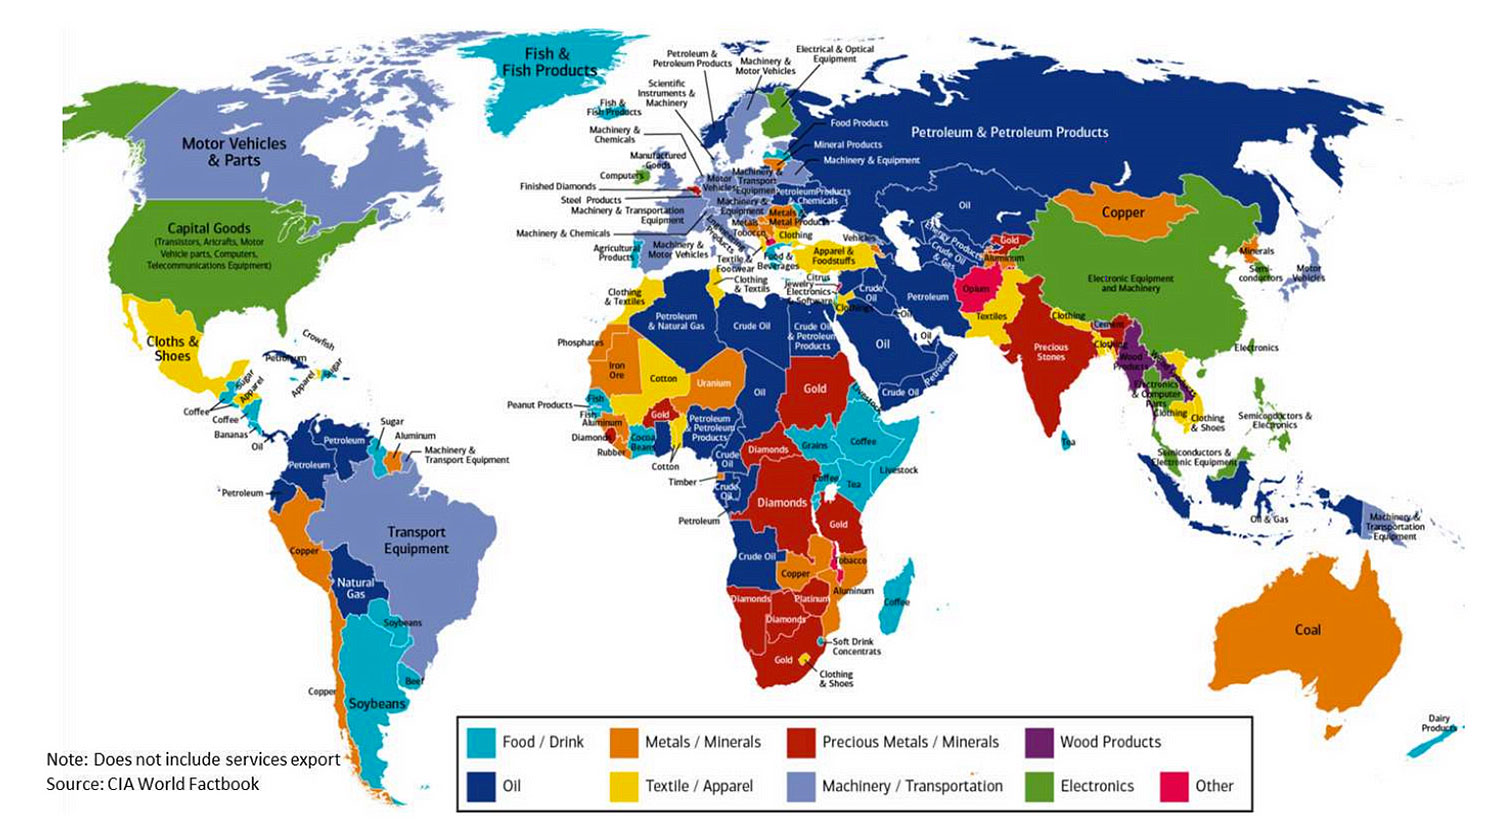
\includegraphics[scale=0.3]{img/exportbycountry}
\end{frame}

\begin{frame}[shrink=20]{Current account of Russian Federation}{in millions of US dollars for period from 2005 to 1Q 2014}
% Table generated by Excel2LaTeX from sheet 'Лист2'
\begin{table}[htbp]
  \centering
  \begin{tabularx}{\linewidth}[b]{@{}>{\raggedright\arraybackslash}Xrrrrr@{}}
    \toprule
%    \rowcolor{green}
    Indicator & \multicolumn{1}{c}{2005} & \multicolumn{1}{c}{2008} & \multicolumn{1}{c}{2011} & \multicolumn{1}{c}{2013} & \multicolumn{1}{c}{Q1 2014} \\
    \midrule
    \Large{Current account} & \textbf{84389} & \textbf{103935} & \textbf{97274} & \textbf{34141} & \textbf{27089} \\
    \midrule
	\rowcolor{gray!20}    Goods and services & 104560 & 157206 & 163398 & 123661 & 40022 \\
    \small{	      Goods} & 116185 & 177625 & 196854 & 181939 & 50728 \\
	\small{	      Services} & -11626 & -20420 & -33456 & -58277 & -10707 \\
	\rowcolor{gray!20}    Primary income & -18526 & -46483 & -60399 & -80246 & -10998 \\
    \small{	      Compensation of employees} & -1133 & -14357 & -9522 & -13170 & -2361 \\
	\small{	      Investment income} & -17394 & -32125 & -51031 & -67157 & -8664 \\
	\rowcolor{gray!20}    Secondary income & -1645 & -6788 & -5725 & -9274 & -1935 \\
    \bottomrule
    \end{tabularx}%
  \label{tab:addlabel}%
\end{table}%

\raggedright
Source: Central Bank of Russian Federation, www.cbr.ru. 2014.  \end{frame}

\begin{frame}[shrink=20]{Current account of Russian Federation}{in millions of US dollars for period from 2005 to 1Q 2014}
\begin{center}
\begin{figure}
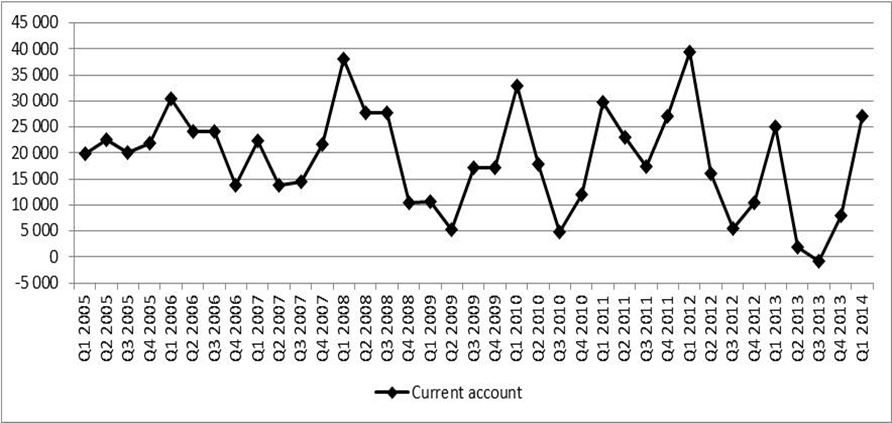
\includegraphics[scale=0.60]{img/curaccount}
\end{figure}
\end{center}
\end{frame}

\begin{frame}[shrink=20]{Capital account of Russian Federation}{in millions of US dollars for period from 2005 to 1Q 2014}
\begin{table}[htbp]
  \centering
\begin{tabularx}{\linewidth}[b]{@{}>{\raggedright\arraybackslash}Xrrrrr@{}}  
    \toprule
    \multicolumn{1}{c}{\textbf{Indicator}} & \multicolumn{1}{c}{\textbf{2005}} & \multicolumn{1}{c}{\textbf{2008}} & \multicolumn{1}{c}{\textbf{2011}} & \multicolumn{1}{c}{\textbf{2013}} & \multicolumn{1}{c}{\textbf{Q1 2014}} \\
    \midrule
    \Large{Capital account} & \textbf{-12387} & \textbf{-104} & \textbf{130} & \textbf{-395} & \textbf{-185} \\
    \midrule
    acquisitions (debit) /disposals (credit) of nonproduced nonfinancial assets  & -57   & -309  & 38    & -146  & -191 \\
    Capital transfers & -12331 & 205   & 92    & -249  & 6 \\
	General government & -12331 & 205   & 4     & -430  & -47 \\
    Financial corporations, nonfinancial corporations, households & 0     & 0     & 88    & 181   & 53 \\
    \bottomrule
    \end{tabularx}%
  \label{tab:addlabel}%

\raggedright
Source: Central Bank of Russian Federation, www.cbr.ru. 2014.  
\end{table}%

\end{frame}

\begin{frame}[shrink=20]{Financial account of Russian Federation}{in millions of US dollars for period from 2005 to 1Q 2014}
\begin{table}[htbp]
  \centering
  \begin{tabularx}{\linewidth}[b]{@{}>{\raggedright\arraybackslash}Xrrrrr@{}}
    \toprule
    Indicator & \multicolumn{1}{c}{\textbf{2005}} & \multicolumn{1}{c}{\textbf{2008}} & \multicolumn{1}{c}{\textbf{2011}} & \multicolumn{1}{c}{\textbf{2013}} & \multicolumn{1}{c}{\textbf{Q1 2014}} \\
    \midrule
    \Large{Financial account} & \textbf{66997} & \textbf{100781} & \textbf{88748} & \textbf{22906} & \textbf{21229} \\
    \midrule
    Direct investment  & 2372  & -19120 & 11767 & 16058 & 5627 \\
    Portfolio investment  & 11443 & 35691 & 15277 & 11011 & 17635 \\
    Financial derivatives & 233   & 1370  & 1394  & 346   & 623 \\
    Other investment  & -8511 & 121765 & 47679 & 17567 & 24695 \\
    Reserve assets  & 61461 & -38925 & 12630 & -22077 & -27351 \\
    \midrule
    \Large{Net errors and omissions} & \textbf{-5004} & \textbf{-3051} & \textbf{-8655} & \textbf{-10840} & \textbf{-5675} \\
    \bottomrule
    \end{tabularx}%
  \label{tab:addlabel}%

\raggedright
Source: Central Bank of Russian Federation, www.cbr.ru. 2014.
\end{table}%
\end{frame}

\begin{frame}[shrink=20]{Balance of payments of Russian Federation}{in millions of US dollars for period from 2005 to 1Q 2014}
\begin{table}[htbp]
  \centering
  \begin{tabularx}{\linewidth}[b]{@{}>{\raggedright\arraybackslash}Xrrrrr@{}}
    \toprule
    Indicator & \multicolumn{1}{c}{-2005-} & \multicolumn{1}{c}{-2008-} & \multicolumn{1}{c}{-2011-} & \multicolumn{1}{c}{-2013-} & \multicolumn{1}{c}{Q1 2014} \\
    \midrule
    Current account & 84389 & 103935 & 97274 & 34141 & 27089 \\
    Capital account & -12387 & -104  & 130   & -395  & -185 \\
    Financial account* & -66997 & -100781 & -88748 & -22906 & -21229 \\
    Net errors and omissions & -5004 & -3051 & -8655 & -10840 & -5675 \\
    Total** & 1     & -1    & 1     & 0     & 0 \\
    \bottomrule
    \end{tabularx}%
    \caption*{Source: Central Bank of Russian Federation, www.cbr.ru. 2014.
    
    * Financial account is reported in previous tables with opposite sign. In fact it must be subtracted from the current account.
    
** Total sum not always equals to zero because of rounding errors.}
  \label{tab:addlabel}%
\end{table}%
\end{frame}
\begin{frame}{}
\begin{block}{The balance of payments identity}
Expressed with the IMF definition, the balance of payments identity can be written:

Current account + Capital account + Financial account + Balancing Item = 0
\end{block}

\end{frame}
\subsection{The BoP transactions classification}
\begin{frame}{The balance of payments transactions classification}
\begin{itemize}[<+->]
\item
The balance of payments is composed as a balance sheet using double-entry bookkeeping – every item involves two entries, a credit and a debit. 
\item
The credits record items lead to payments inflows. Such items are associated with a greater demand for domestic currency or supply of foreign currency to the foreign exchange market. 
\item
The debits record items lead to payments outflows. These are associated with a greater supply of domestic currency or demand for foreign currency in the foreign exchange market.
\end{itemize}
\end{frame}
\setbeamercovered{invisible}
%\setbeamercovered{transparent}
\begin{frame}[shrink=25]{Balance of Payments example operations}{thousands USD}
\small
\begin{table}[H]
    \begin{tabular}{lr|lr}
    %\begin{tabular}{p{4cm}p{1.5cm}|p{4cm}p{1.5cm}}
        \hline
        Current account &Credit $(+)$&Debit $(-)$&\\
        \hline
        \hiddencell{3}{Goods} 	& \hiddencell{3}{5000(2)}&  \hiddencell{5}{Services }& \hiddencell{5}{25(4)}\\
        \hiddencell{4}{Investment income}& \hiddencell{4}{25(3)} &  &\\
        \hiddencell{6}{Goods}& \hiddencell{6}{50(5)}& & \\
              & & & \\
              & & & \\
        \hline
        \textbf{Net   }& \hiddencell{8}{\textbf{5050}}& \textbf{Net }&\\
        \hline
    	Capital account &Credit $(+)$&Debit $(-)$&\\
        \hline
        \hiddencell{2}{Corporations\&households} & \hiddencell{2}{5000(1)} 
        & \hiddencell{2}{Corporations\&households} & \hiddencell{2}{5000(1)} \\
        \hiddencell{5}{Corporations\&households} & \hiddencell{5}{25(4)}
		& \hiddencell{3}{Corporations\&households} & \hiddencell{3}{5000(2)}\\
        & & \hiddencell{4}{Corporations\&households}& \hiddencell{4}{25(3)}\\
        & & \hiddencell{6}{Capital transfers}& \hiddencell{6}{50(5)}\\
        & & \hiddencell{7}{Corporations\&households}& \hiddencell{7}{50000(6)}\\
        \hline
        \textbf{Net   }& & \textbf{Net }&\hiddencell{9}{\textbf{55050}}\\
        \hline
        Financial account &Credit $(+)$&Debit $(-)$&\\
        \hline
        \hiddencell{7}{Reserve assets} 	&\hiddencell{7}{50000(6)} &&\\
        & & & \\
        \hline
         \textbf{Net   }& \hiddencell{10}{\textbf{50000}} & \textbf{Net }&\\
        \hline
    Balance of payments &Credit $(+)$&Debit $(-)$&\\
        \hline
        \hiddencell{11}{Current account} & \hiddencell{11}{5050} & \hiddencell{11}{Capital account} & \hiddencell{11}{55050}\\
              \hiddencell{11}{Financial account} & \hiddencell{11}{50000} &&\\
        \hline
        \textbf{Net}    & \hiddencell{12}{\textbf{0}} &\textbf{Net} &\\
        \hline
    \end{tabular}
    \label{tab:bop}	
\end{table}
\normalsize

\end{frame}
\setbeamercovered{transparent}

\subsection{BoP Equilibrium and Adjustment}
\begin{frame}{Balance of Payments Equilibrium and Adjustment}
\begin{itemize}[<+->]
\item
Balance of payments equilibrium exists when exports equal imports or credits equal debits on some particular subaccount. 
\item
In the case of flexible exchange rates balance of payments equilibrium is restored by the operation of the free market. 
\item
When the exchange rate is fixed the national currency can be overvalued or undervalued and the central banks must now finance the trade imbalance by international reserve flows.
\item
Central banks use direct controls on international trade sometimes.
\end{itemize}
\end{frame}

\begin{frame}{China is growing its importance}
\begin{figure}
	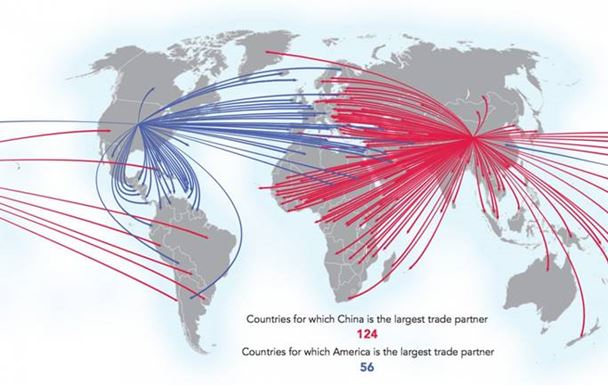
\includegraphics[scale=0.5]{img/China_US_Trade_Partners}
\end{figure}
Sources: Khanna, P. (2016). Connectography: mapping the future of global civilization. Random House.
\end{frame}

\subsection{The Russian Foreign Debt}
\begin{frame}[shrink=30]{External Debt of the Russian Federation as of  December 2015 (estimate)}{(millions of US dollars)}

% Table generated by Excel2LaTeX from sheet 'Лист1'
\begin{table}[htbp]
  \centering
  \begin{tabularx}{\linewidth}[b]{@{}>{\raggedright\arraybackslash}Xrrr@{}}
    \toprule
          & Dec. 2013 &  Dec. 2014 &  Dec. 2015 \\
    \midrule
    Total & 728864 & 599041 & 515254 \\
    \midrule
    1. General Government & 61743 & 41606 & 30743 \\
    1.1. Federal Government & 60962 & 41027 & 30180 \\
    1.1.1. New Russian Debt & 58949 & 39257 & 28939 \\
    1.1.2. Debt of the former USSR & 2012  & 1770  & 1241 \\
    1.2. Local Government & 781   & 580   & 563 \\
    2. Central bank & 15963 & 10599 & 11528 \\
    3. Banks & 214394 & 171450 & 132349 \\
    4. Other sectors & 436764 & 375386 & 340633 \\
    4.1. Debt liabilities to direct investors and to direct investment enterprises & 151288 & 133451 & 130303 \\
    4.2. Loans and deposits & 268402 & 225978 & 197559 \\
    4.3. Debt securities & 9155  & 6145  & 4736 \\
    4.4. Trade credits & 3115  & 3469  & 2812 \\
    4.5. Financial leases & 2105  & 2433  & 2501 \\
    4.6. Other  & 2700  & 3909  & 2722 \\
    \bottomrule
    \end{tabularx}%
  \label{tab:addlabel}%
  
  \raggedright
  Source: Central Bank of Russian Federation, www.cbr.ru. 2016.
\end{table}%
\end{frame}


\end{document}